\documentclass[../review_3.tex]{subfiles}
\graphicspath{{\subfix{../img/}}}
\begin{document}

\chapter{Auswertung des Projekts}\thispagestyle{fancy}
Während der letzten Phase des Softwareprojektes wurden zwei anonyme Umfragen mithilfe des Umfragetools LimeSurvey erstellt, durchgeführt und ausgewertet. Deren Ergebnisse werden in diesem Kapitel aufgezeigt und näher erläutert.
\section{Kritische Bewertung des Projekterfolgs}
Das folgende Teilkapitel bezieht sich auf die Bewertung des Projekterfolgs. Die weiteren Teilkapitel sind dem Vorgehen und den sonstigen Ergebnissen der Umfrage gewidmet.
%
% Hier kann man bestimmt noch mehr schreiben, wenn das Teilkapitel vervollständigt worden ist
%
\subsection{Einhaltung der in der Planungs- und Entwurfsphase beschlossenen Werte}
Zu Beginn des Projekts wurde sich auf acht (agile) Werte geeinigt (vgl. Abb \ref{werte}), die unter anderem im Gitlab-Wiki und im ersten Reviewdokument festgehalten wurden. Diese Werte sollten die bestmögliche Zusammenarbeit im Team gewährleisten.
\begin{figure} [t]
    \centering
    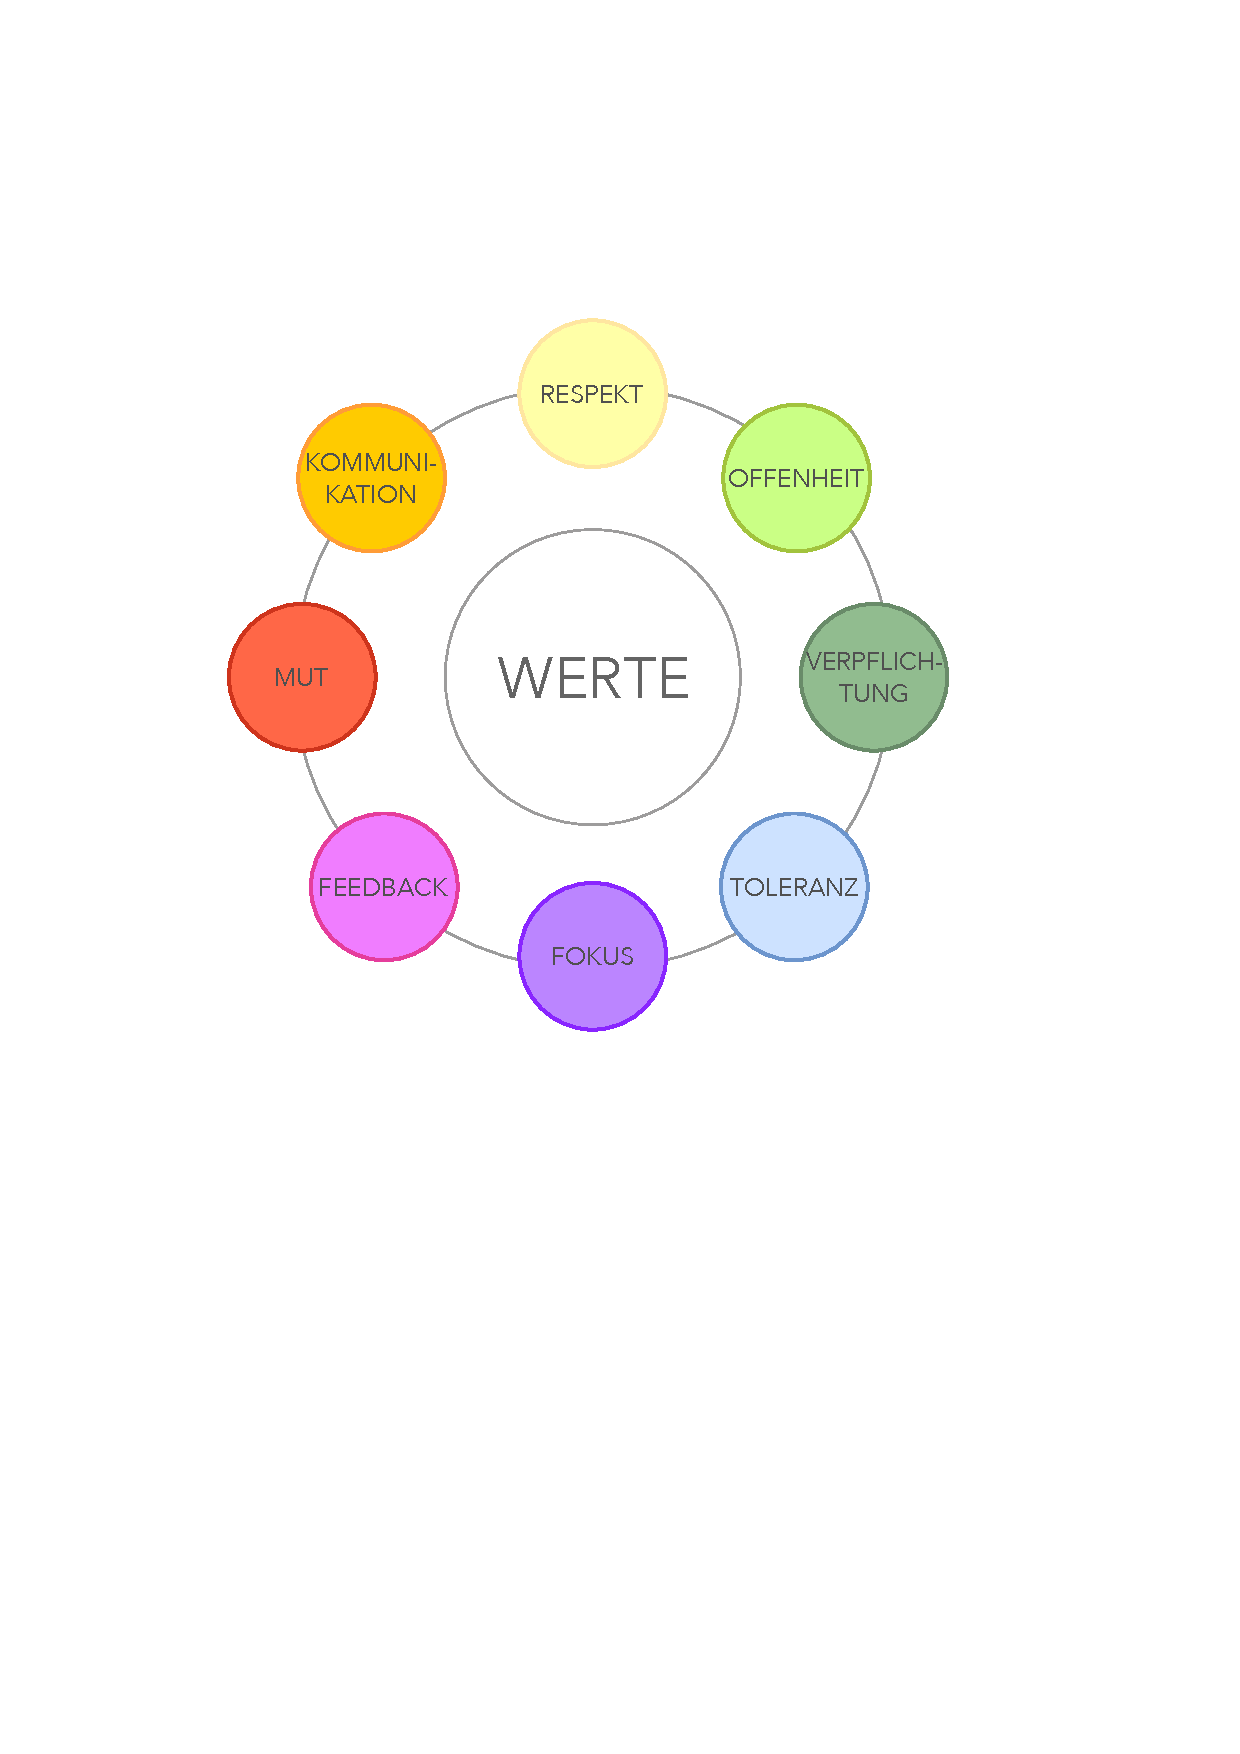
\includegraphics[width = 0.7\linewidth]{img/Werte.pdf}
    \caption{Die in der Planungs- und Entwurfsphase beschlossenen Werte}
    \label{werte}
\end{figure}

Im Folgenden werden die gemeinsam beschlossenen Werte kurz erklärt:

Jedes Teammitglied zeigt den anderen Studierenden \textbf{Respekt} und schätzt diese. Außerdem soll jedem Verständnis entgegengebracht werden, zum Beispiel wenn eine Person Probleme hat. Zudem soll auf Schwächere Rücksicht genommen werden.

\textbf{Offenheit} bedeutet hier, dass neue Informationen und Erfahrungen bewusst aufgenommen und nicht vorschnell als unwichtig bewertet werden. Jeder darf seine Meinung frei äußern, um Missverständnissen und Auseinandersetzungen vorzubeugen. Ebenso soll Transparenz herrschen und Problemen soll sofort auf den Grund gegangen werden.

Der Wert \textbf{Verpflichtung} kann so interpretiert werden, dass alle Teammitglieder sich der Projektaufgabe verbunden fühlen sollen.

Außerdem sind \textbf{Toleranz} und Vielfalt zentrale Werte. Personen mit anderen Sichtweisen werden nicht etwa als Konkurrenten gesehen, sondern vielmehr als Bereicherung für das Team.

Der \textbf{Fokus} liegt im Projekt vor allem auf den Aufgaben und den gemeinsamen Zielen. Verschwenden von Zeit und Kapazitäten sowie Ablenkungen sollen vermieden werden. Zudem hat die Fertigstellung einer bereits begonnen Aufgabe Vorrang gegenüber dem Start einer neuen Aufgabe.

Indem in den Meetings regelmäßig der derzeitige Stand aufgezeigt wird, kann sich jedes Teammitglied individuelles \textbf{Feedback} von den anderen Beteiligten holen.

Zusätzlich soll jedes Teammitglied \textbf{Mut} aufweisen, indem es zum Beispiel neue Aufgaben übernimmt, auch wenn sie zuerst als schwer machbar und komplex erscheinen. Außerdem erfordert es Mut zu sagen, wenn Hilfe benötigt wird, oder auch mitzuteilen, wenn eine Aufgabe länger als zuvor erwartet dauert. Auch das Ausprobieren neuer Lösungswege fällt unter den Wert Mut.

Zudem ist die tägliche \textbf{Kommunikation} mit den Teammitgliedern für eine gute Zusammenarbeit erforderlich. So sollte jeder mehrmals täglich nach neuen Zulip-Nachrichten schauen und dort auf Fragen anderer antworten. Außerdem wurde gemeinsam beschlossen, dass bei Änderungen an Dokumenten andere benachrichtigt werden.

In der durchgeführten Umfrage sollte von den Teilnehmenden bewertet werden, wie stark die einzelnen Werte ihrem Ermessen nach während des Projekts beachtet wurden. Die Zahl 1 stand hierbei für \glqq sehr wenig\grqq{}, 2 für  \glqq wenig\grqq{}, 3 für  \glqq teils-teils\grqq{}, 4 für  \glqq stark\grqq{} und die Zahl 5 für  \glqq sehr stark\grqq{}.

\begin{figure} [t]
    \centering
    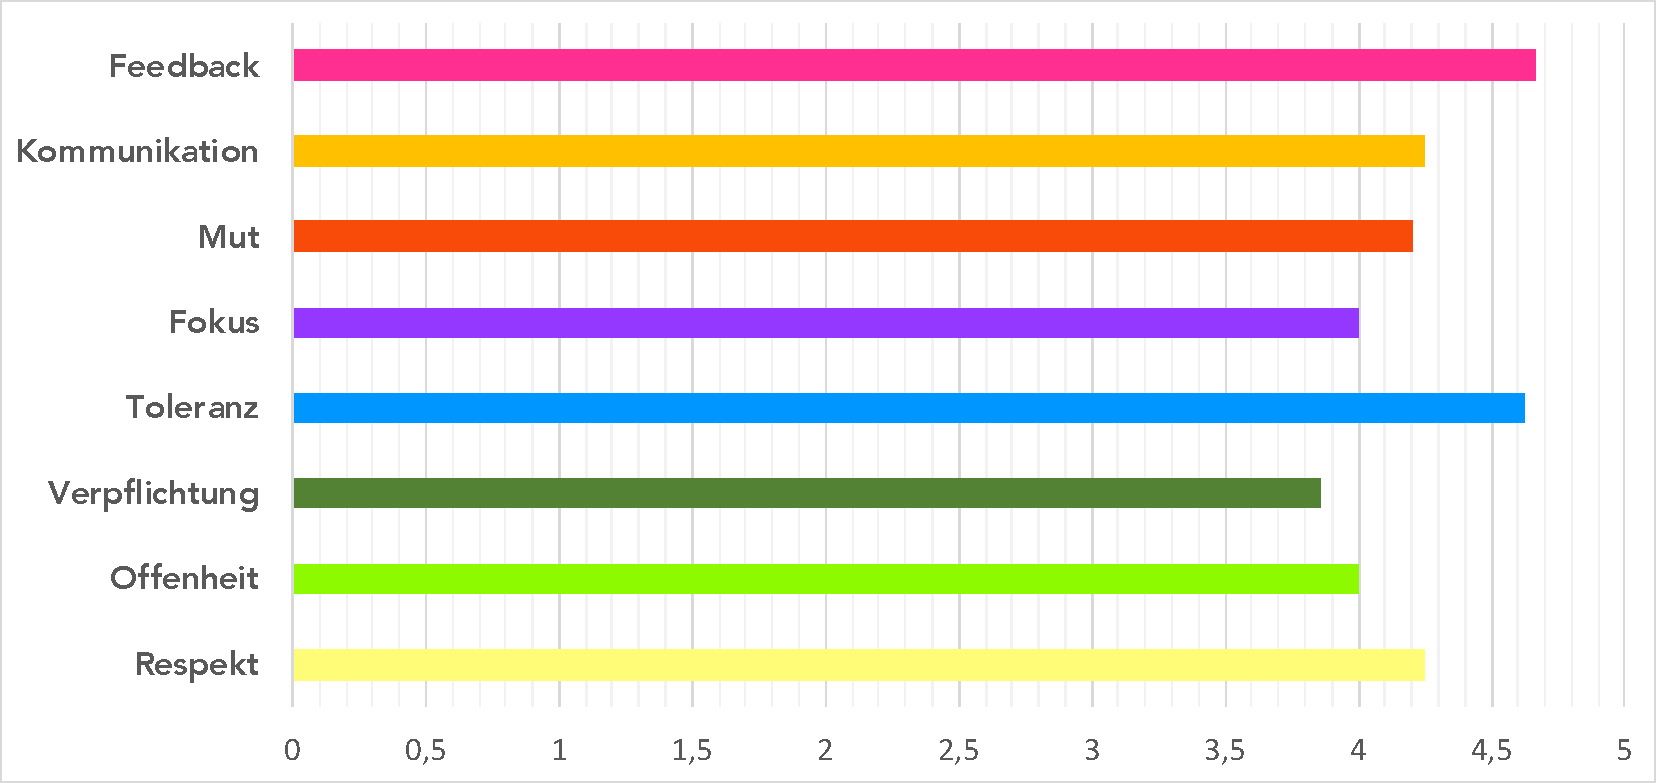
\includegraphics[width = \linewidth, trim=8pt 8pt 8pt 8pt, clip]{img/werteErg.pdf}
    \caption{Klassifizierung der Einhaltung der Werte}
    \label{werte2}
\end{figure}

Das Ergebnis der Umfrage zeigt, dass nach Meinung der Teammitglieder alle Werte stark bzw. sehr stark beachtet wurden. Die geringste Klassifizierung hat die \textbf{Verpflichtung} mit einem Wert von 3,857. Jedoch ist dieser Wert immer noch gut und sehr nahe an ,,stark''. Vor allem der Wert \textbf{Toleranz} hat mit einer durchschnittlichen Klassifizierung von 4,625 einen sehr hohen Wert erhalten. Dies zeigt, dass die Teammitglieder ihre Kommilitonen in der Gruppe nicht als Konkurrenten sahen, sondern vielmehr als Bereicherung für das gesamte Team.

\subsection{Zufriedenheit des Teams mit dem bisherigen Projekterfolg}
Circa anderthalb Wochen vor Projektabgabe wurden die Projektteilnehmer nach deren Zufriedenheit mit dem bisherigen Stand des Projekts gefragt.
Nach den Ergebnissen dieser Umfrage äußerten vier Personen, zufrieden zu seien, zwei jedoch nur teilweise.
Es sollte nun versucht werden, die Zufriedenheit des Teams in der restlichen Zeit deutlich zu erhöhen.

\section{Kritische Bewertung des Vorgehens}
Eine Aussage, die unter anderem eine der beiden Umfragen beinhaltete, lautete: \glqq Die Wahl des Unified Process war die richtige.\grqq{} Alle acht Teilnehmer dieser Umfrage stimmten dieser Aussage zu. Zudem gab eine Person an, dass das tatsächliche Vorgehen im Projekt voll und ganz dem des Unified Process entsprach. Die restlichen sieben Teilnehmer machten als Angabe, dass das tatsächliche Vorgehen stark dem des Unified Process entsprach.

Positiv ist außerdem zu bewerten, dass vier der acht Teammitglieder nach Auswertung der Umfrage daran interessiert sind, auch nach Ende der Lehrveranstaltung noch weiter am Projekt zu arbeiten.

In der Umfrage wurde außerdem gefragt, inwieweit der einzelne Teilnehmer mit seiner Rolle zufrieden sei. Diese Rollen wurden bereits im ersten Meeting des Projekts verteilt.
Zwei Teilnehmer seien mit ihrer Rollenzuteilung sehr zufrieden, vier weitere zufrieden. Lediglich zwei gaben zur Angabe, dass sie mittelstark mit dieser Zuteilung zufrieden seien.

\subsection{Probleme}
In der Umfrage wurde auch nach Problemen gefragt, die nach Meinung des Teilnehmers bzw. der Teilnehmerin im Softwareprojekt auftraten. Die Teilnehmenden konnten zu den einzelnen aufgeführten Problemen einen Kommentar hinterlassen oder ein zusätzliches Problem, welches noch nicht aufgeführt wurde, hinzufügen und näher erläutern.

\begin{longtable}[h]{p{6,7cm} c}
    \toprule
    \textbf{In der Umfrage aufgeführtes Problem}                            & \textbf{Ja-Stimmen/Anzahl der Teilnehmenden} \\ \midrule \endhead
    Fehlende Absprache innerhalb der Projektgruppe/ schlechte Kommunikation & 4/8                                          \\
    Schwierigkeiten bei der Entscheidungsfindung innerhalb der Gruppe       & 2/8                                          \\
    Fehlende Informationen                                                  & 1/8                                          \\
    Zeitmangel                                                              & 4/8                                          \\
    Unklare Projektziele                                                    & 0/8                                          \\
    Schlechte Stimmung innerhalb des Teams                                  & 1/8                                          \\
    Unterschätzte Komplexität                                               & 3/8                                          \\
    Mangelnde Unterstützung seitens der Uni                                 & 2/8                                          \\ \bottomrule
\end{longtable}

Bei dieser Abstimmung wurde von einem Teilnehmer darauf hingewiesen, dass es zu Beginn bei der Absprache innerhalb der Projektgruppe und bei der Kommunikation Probleme gab. Jedoch sei dies jetzt besser geworden. Zudem wäre nach Angaben eines anderen Studierenden folgende Situation aufgetreten: \glqq A wartet, dass B fertig wird, aber B braucht Anforderungen von A\grqq{}. Eine andere Person empfand vor allem zu Beginn bis zur frühen Mitte des Projekts die Situation als nicht ganz durchsichtig, vor allem im Bezug darauf, wie der Stand einzelner Personen war. Der Grund sei aber vor allem darin zu begründen, dass jeder viele verschiedene Aufgaben zu erledigen hätte und so nur das Wichtigste in den Meetings verkünden konnte. Ein weiterer möglicher Grund für mangelnde Kommunikation während der Anfangsphase des Projektes könnte darin begründet sein, dass sich die Teilnehmer untereinander noch kaum kannten, und ein normales Kennenlernen aufgrund der Pandemiesituation nicht möglich war.

Zu Beginn beim Bau der Diagramme seien Schwierigkeiten bei der Entscheidungsfindung innerhalb der Gruppe aufgetreten. Außerdem seien teilweise unnötige Debatten geführt worden.

Als ein großes Problem wurde von den Teilnehmenden der Zeitmangel gesehen. Das Semester sei zu voll. Das Softwareprojekt sollte aber nach Meinung dieser einen Person nicht weniger Zeit in Anspruch nehmen, sondern vielmehr andere Kurse. Eine andere Person war der Auffassung, dass es zu viele Module in diesem Semester gäbe. Sie hätte zwar keine Wiederholungen offen und gäbe ihr Bestes, trotzdem sei das Projekt sehr aufwendig. Auch wurde kritisiert, dass zum Zeitpunkt der Umfrage die zweite Phase längst beendet sei, jedoch das Produkt AEGIS immer noch nicht richtig funktioniere. Ein anderer Mitstreiter wiederum sah weniger das Problem im Zeitmangel, sondern eher in den vorgegeben 20h, die meist überschritten werden mussten.

Von einem wurde auch die unterschätzte Komplexität, vor allem in Hinsicht auf die Klasse \texttt{PacketInfo}, und die mangelnde Unterstützung seitens der Universität als Problem gesehen. Er fragte sich, ob die Teilnehmer wirklich bereit für ein solches Projekt seien oder ein großer Teil von denjenigen gemacht wurde, die schon vor der Uni über Wissen verfügten. Jemand anders würde gerne mehr bzw. andere Softwarelizenzen von der Universität zur Verfügung gestellt bekommen. Seiner Meinung nach sei zudem die Komplexität durch mangelndes Wissen über die Bedingungen, die Programmiersprache und die generellen Konstrukte erhöht worden.

Eine Person äußerte Probleme bezüglich fehlender Informationen und einer schlechte Stimmung innerhalb des Teams. So wäre es für sie interessant gewesen, über die genauen Umgebungsparameter informiert zu sein. Ihrer Meinung nach hätte es zwar am Anfang eine noch größere Belastung mit sich gebracht, jedoch sei es dann vielleicht planbarer gewesen. Auch spürte sie teilweise schlechte Laune in Meetings. Die Ursache sah sie im Stress. Hier soll angemerkt werden, dass lediglich ein Teilnehmender diese beiden Punkte als Problem sah.

Unklare Projektziele innerhalb des Teams wurde von keinem als Probleme identifiziert.

Auch wenn einige Probleme, die wahrscheinlich auf der Unerfahrenheit vieler Projektbeteiligten ruhten, während der Ausführung des Projektes auftraten, wurden diese im Laufe der Zeit reduziert beziehungsweise komplett gelöst. Dies soll hier positiv angemerkt werden und spricht für die Offenheit und Flexibilität des Teams.

\subsection{Meetings}

Es war den Umfrageteilnehmern möglich, eigene Anmerkungen zum Thema \glqq Meetings\grqq{} hinzuzufügen.
So hielt ein Teilnehmer die internen Meetings am Anfang für etwas lang und unorganisiert, jedoch hätten sich diese Dinge im Laufe der Zeit stark verbessert. Er würde die Meetings mittlerweile als das unter diesen Umständen Bestmögliche bezeichnen. Für eine weitere Person waren ebenso die Meetings mit dem Betreuer Martin Backhaus sehr wichtig und hilfreich. Ihre Unberechenbarkeit in puncto Länge störte diese aber. Denn ihrer Meinung nach wären die Montagsmeetings häufig sehr lange gewesen, während das Meeting am darauffolgenden Donnerstag meist nur eine halbe Stunde andauerte. Dies sei ungünstig, da am Donnerstag alle Teilnehmer drei Stunden Zeit haben.

Eine weitere Anmerkung bezog sich auf vielmehr auf die Frage, ob Online-Meetings Treffen in Präsenz völlig ersetzen könnten. Hier wurde angemerkt, dass durch Meetings in Präsenz Absprachen wahrscheinlich leichter zu treffen wären, sowie die Kommunikation einfacher gewesen wäre. Außerdem würden eventuell Fehler schneller aufgedeckt worden sein. Zudem würden die Online-Meetings das Bilden eines Teamgefühls erschweren. Generell wäre nach Auffassung dieses Umfrageteilnehmenden das Testen am Testbed durch die direkte Anwesenheit bei Präsenzlehre um einiges einfacher gewesen.

Trotz allem wurde an den viermal wöchentlichen Meetings zahlreich teilgenommen. Von KW 17 bis KW 27 fanden insgesamt 36 Meetings statt. Von diesen 36 Meetings war der Betreuer an 20 anwesend. Die restlichen Treffen fanden gruppenintern statt.

\begin{figure} [h]
    \centering
    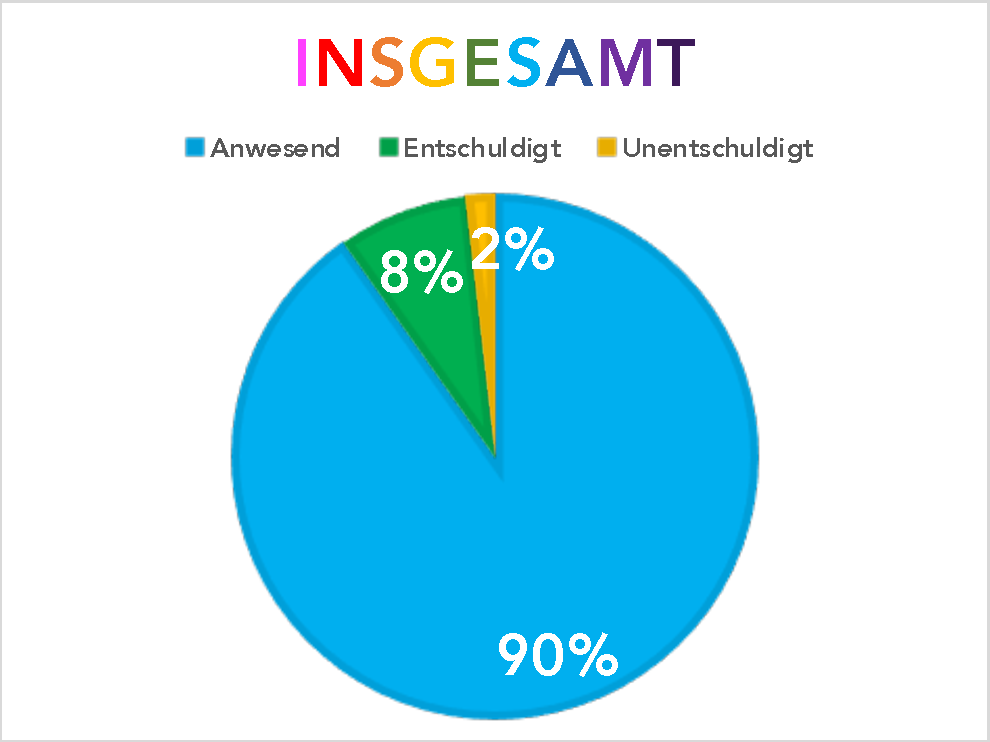
\includegraphics[width = 0.5\linewidth, trim=10pt 10pt 10pt 10pt, clip]{img/insgesamt.pdf}
    \caption{Durchschnittliche Anwesenheit}
    \label{ins}
\end{figure}

Insgesamt waren an den Meetings 90,24\% der Teammitglieder anwesend (vgl. Abb. \ref{ins}). An 8,03\% fehlt jemand entschuldigt und bei 1,73\% unentschuldigt.

\begin{figure} [H]
    \centering
    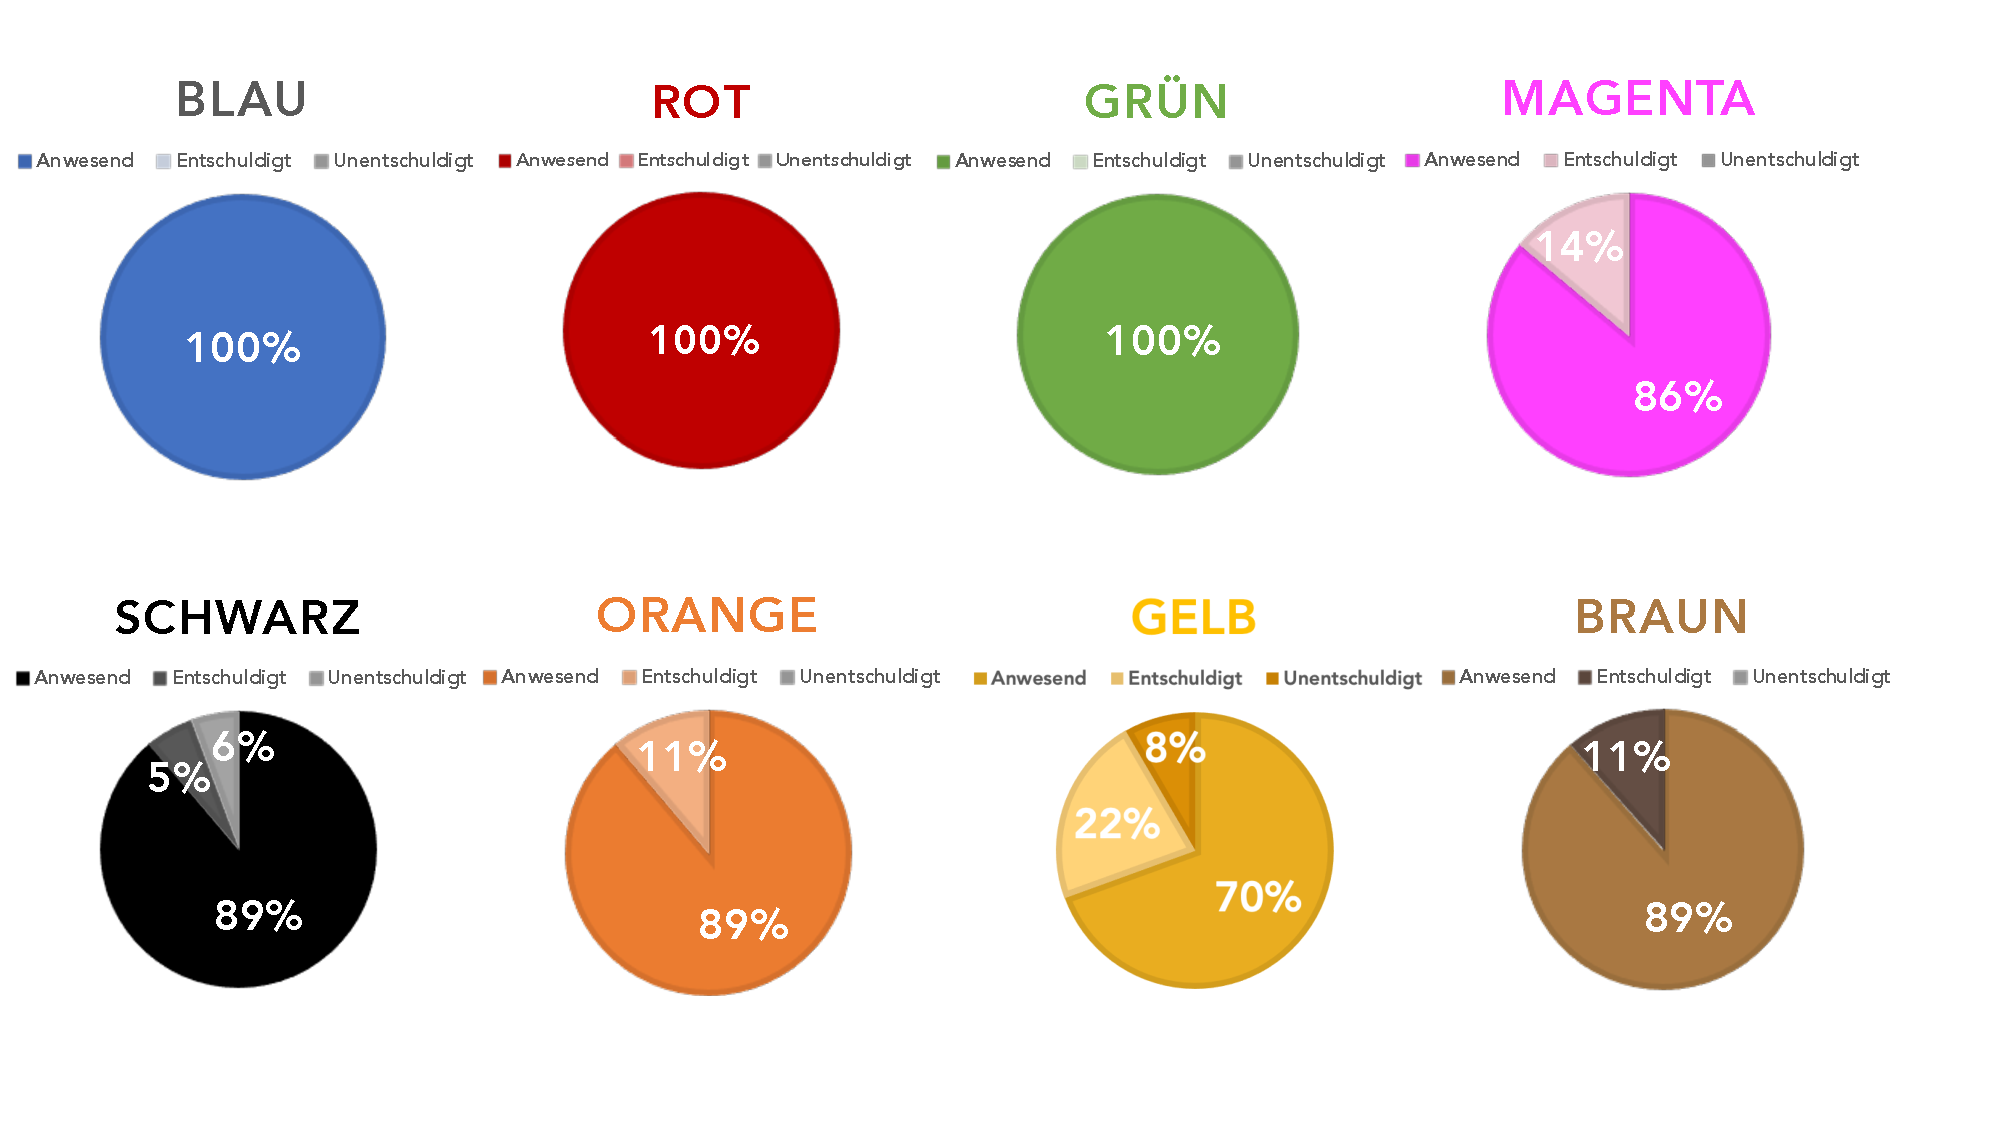
\includegraphics[width = \linewidth]{img/meetingsstatstik.pdf}
    \caption{Vergleich der Anwesenheit zwischen den unterschiedlichen Projektteilnehmern}
    \label{stat}
\end{figure}

Drei der acht Projektteilnehmer waren an allen 36 Meetings anwesend. Weitere drei Personen waren an 89\% anwesend. Die Anwesenheitsquote eines weiteren Teammitglieds liegt mit 86\% nur knapp darunter. Am seltesten war die \glqq gelbe\grqq{} Person anwesend. Von den Personen, die an manchen Terminen fehlten, hat sich der Großteil zuvor bei der Projektleiterin entschuldigt.

Anmerkung: Es wurden für die einzelnen Personen die gleichen Farben gewählt wie bei der Kimai-Auswertung in Kapitel 7.

\subsection{Eintreten von Risiken} %fragen bei nächster Umfrage

Folgende Risiken wurden in der Planungs- und Entwurfsphase identifiziert:

\begin{longtable}[h]{l p{2,5cm} p{2,5cm} p{3,5cm} p{3,5cm}}
    \toprule
    \textbf{ID} & \textbf{Risiko}                                                                                                                                           & \textbf{Eintrittswahr-scheinlichkeit} & \textbf{Auswirkung}                                                                                                                                              & \textbf{Maßnahmen}                                                                                                                                                                                                           \\ \midrule \endhead
    R01         & Software wird unzureichend dokumentiert.                                                                                                                  & 30\%                                  & Sicherheitslücken, falsch aufgefasste Anforderungen, Softwareanomalien, schwierige Wartung, Software kann nicht richtig getestet werden u. v. m.                 & Motivation der Teammitglieder dazu, dass diese gewissenhaft Dokumentation führen; Erklären der Wichtigkeit der Dokumentation; Einführen von Konventionen zur Dokumentation; Verwendung automatischer Dokumentationswerkzeuge \\
    R02         & Unzureichende Erfahrung des Projektteams bezüglich neuer Tools (z. B. DPDK, Ninja, Meson) und der Programmiersprache C++                                  & 80\%                                  & Zeitverzögerung (v. a. längere Dauer der Implementierung durch umfassende Einarbeitungsphase)                                                                    & Gute Einarbeitung; Erstellen und Halten von Präsentationen zu schwierigen Themen; Gegenseitige Hilfe; Festlegen von Ansprechpartner für die einzelnen Themenbereiche                                                         \\
    R03         & Weniger Austausch und weniger effiziente Zusammenarbeit durch  Online-Lehre                                                                               & 70\%                                  & Probleme werden später oder nicht sichtbar; schwieriger Überblick über den Arbeitsstand bei anderen Teammitgliedern; Statusmeldungen fehlen; Geringes Teamgefühl & regelmäßige Treffen ohne Zeitdruck; möglichst organisierte Kommunikation (z.B. über Zulip oder Webex)                                                                                                                        \\
    R04         & Hardware-Probleme (z. B. Ausfall oder andere Defekte)                                                                                                     & 20\%                                  & Zeitverzögerung, finanzielle Kosten                                                                                                                              & sorgfältiger Umgang mit der Hardware                                                                                                                                                                                         \\
    R05         & Testbed nicht optimal konfigurierbar (aufgrund der verringerten Geräteanzahl und beschränkter Optionen ist nicht jede vorteilhafte Konstellation möglich) & 60\%                                  & erschwerte Implementierung, Zeitverzögerung, Nichterfüllen einzelner Anforderungen, finanzielle Kosten beim Kauf zusätzlicher Hardware                           & möglichst effiziente Nutzung der vorhandenen Hardware; Kauf zusätzlicher Hardware; Entwicklung eines Netzwerkplans                                                                                                           \\ \bottomrule
\end{longtable}

Abbildung \ref{riskomatrix} visualisiert die in der Planungs- und Entwurfsphase identifizierten Projektrisiken R01 bis R06, indem sie die Eintrittswahrscheinlichkeiten und die dazugehörigen Schadensausmaße ins Verhältnis setzt. Je weiter sich im Diagramm nach rechts bewegt wird, desto höher ist die Eintrittswahrscheinlichkeit. Während diese Wahrscheinlichkeit ganz links bei 0\% liegt, beträgt sie am rechten Rand 100\%. Je weiter oben sich das Risiko im Diagramm befindet, desto größer ist das Schadensausmaß.

\begin{figure} [H]
    \centering
    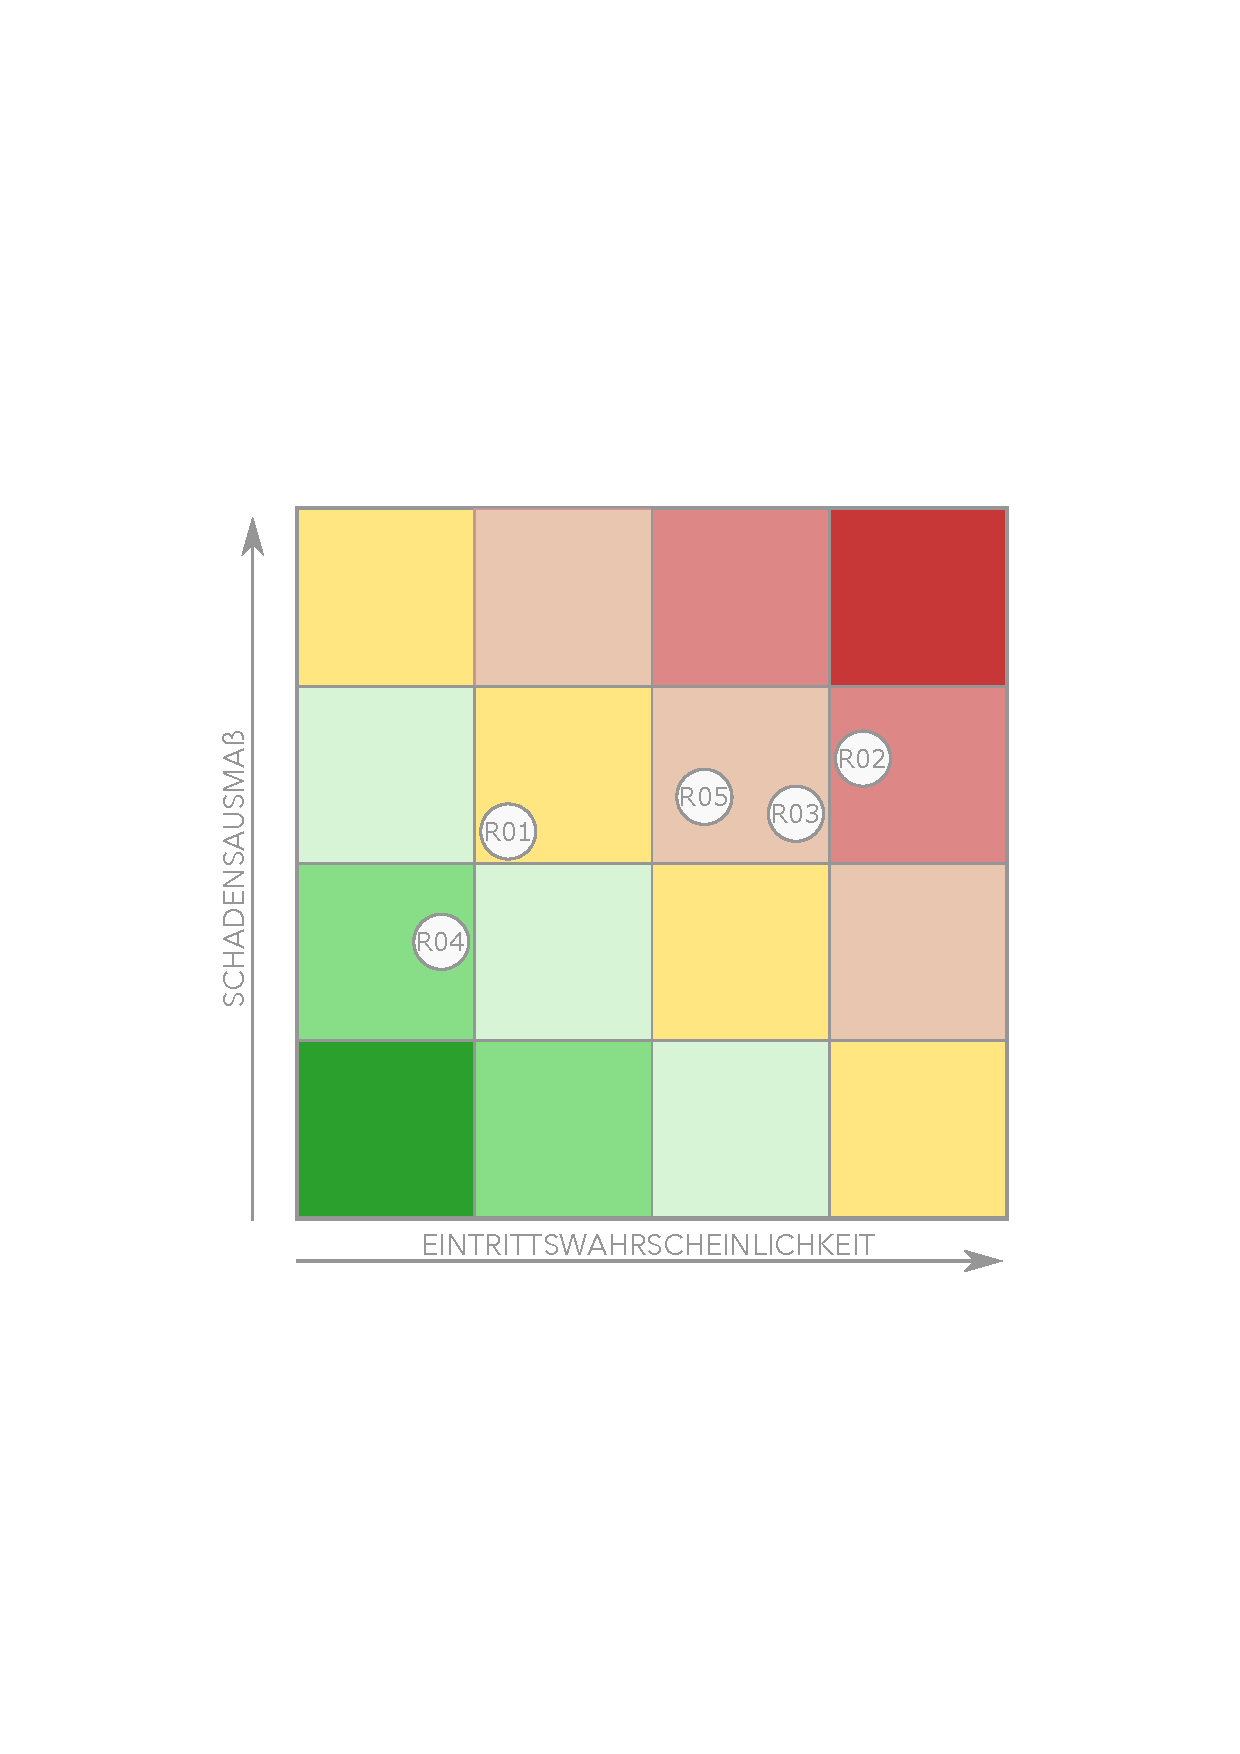
\includegraphics[width = 0.5\linewidth]{img/risikomatrix.pdf}
    \caption{Risikomatrix aus der Planungs- und Entwurfsphase}
    \label{riskomatrix}
\end{figure}

In der zweiten Umfrage sollten die Projektteilnehmer bewerten, welche der oben genannten Risiken aufgetreten sind. Falls ihrer Meinung nach eines dieser Risiken aufgetreten ist, sollten sie kurz erläutern, inwiefern sich das Risiko während des Projektes gezeigt hat und wie stark es den Projekterfolg beeinflusst hat.

\begin{longtable}[h]{p{8.5cm} p{5.3cm}}
    \toprule
    \textbf{Risiko}                                        & \textbf{Anteil der Ja-Stimmen} \\ \midrule \endhead
    \textbf{R01}: Unzureichende Dokumentation              & 0/7                                          \\
    \textbf{R02}: Unzureichende Erfahrung des Projektteams & 5/7                                          \\
    \textbf{R03}: Online-Lehre                             & 2/7                                          \\
    \textbf{R04}: Hardware-Probleme                        & 1/7                                          \\
    \textbf{R05}: Testbed nicht optimal konfigurierbar     & 1/7                                          \\ \bottomrule
\end{longtable}
Niemand der Umfrageteilnehmer war der Meinung, dass sich das Risiko R01 (Unzureichende Dokumentation) während des Projekts gezeigt hat.

Dagegen war über die Hälfte der Teilnehmer der Ansicht, dass dies bei R02 der Fall war. Vor allem die nötige Einarbeitung in DPDK und andere Systeme wie zum Beispiel Meson wurde als sehr arbeitsintensiv und zeitaufwendig empfunden. Auch musste die Projektteilnehmer sich anfangs in die Programmiersprache C++ gewöhnen.

Zwei der drei Umfrageteilnehmer sahen ein Problem in der Online-Lehre (R03).  Dieses Problem wurde aber lediglich als gering eingestuft. Hierbei wurde der fehlende Kontakt außerhalb der \glqq Arbeit\grqq{} und der seltene physische Zugriff auf das Testbed geäußert.

Nur eine Person äußerte sich zum Thema Hardware-Probleme. Bei dieser sei gelegentlich beim Testen und Ausführen von AEGIS der eigene Computer ausgefallen, da dieser nicht so leistungsstark sei. Auch dass das Testbed nicht optimal konfigurierbar sei, ist lediglich von einer Person als gering eingestuft worden. So wurden beispielsweise zur dessen Verwendung Namespaces benötigt worden.

Was sich zeigt, ist, dass Risiko R02, dass schon als Beginn als das mit der höchsten Eintrittswahrscheinlichkeit identifiziert worden war, nach Meinung der meisten Teilnehmenden eingetreten sei. Risiko R01 scheint gar nicht eingetreten zu sein. Die anderen drei Risiken sind durch ihre geringe Auswirkung so gut wie vernachlässigbar.

\subsection{Planungs- und Entwurfsphase}
Die Teilnehmenden wurden zur Zufriedenheit mit dem Ergebnis des ersten Reviewdokuments, der Präsentation und der Diskussion im Anschluss der Präsentation befragt. In Abb. \ref{pr1} sind die Ergebnisse dargestellt.
\begin{figure} [h]
    \centering
    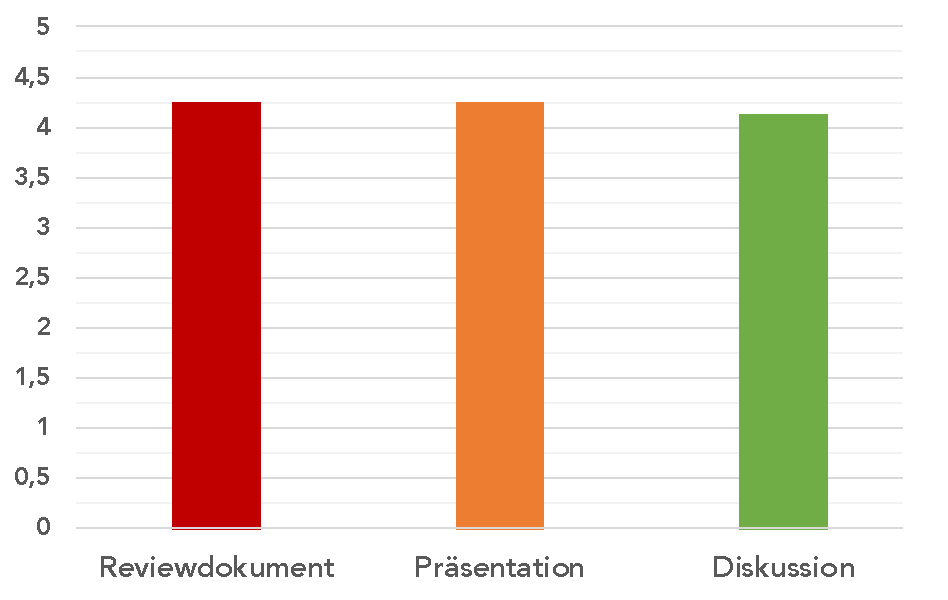
\includegraphics[width = 0.7\linewidth]{img/RevPraeDis1.pdf}
    \caption{Planungs- und Entwurfsphase: Ergebnisse der Bewertung des Reviewdokuments, der Präsentation und der Diskussion im Anschluss}
    \label{pr1}
\end{figure}
Das Reviewdokument wurde von fünf Umfrageteilnehmenden als sehr gut bezeichnet. Weiterhin wurde es von jeweils einer Person mit 2, 3 und 4 klassifiziert, was insgesamt zu einer durchschnittlichen Klassifizierung von 4,25 führt. Auch wenn eine Person mit der Präsentation zur Planungs- und Entwurfsphase vom 27.05.2021 sehr unzufrieden gewesen ist, wurde der Vortrag von allen anderen als gut bzw. sehr gut eingeschätzt und durchschnittlich mit 4,25 klassifiziert. Mit der an die Präsentation anschließenden Diskussion sind alle Befragten mindestens zufrieden gewesen, was bei einer Enthaltung zu einem Durchschnitt von ca. 4,7 führt.

\begin{longtable}[H]{p{6,7cm} p{7,1cm}}
    \toprule
    \textbf{Frage}                     & \textbf{durchschnittliche Klassifizierung durch die Umfrageteilnehmenden} \\ \midrule \endhead
    Zeitliche und psychische Belastung & 2,125                                                                     \\
    Verteilung der Arbeit              & 3,4                                                                       \\ \bottomrule
\end{longtable}

Zwar kann bei den oben beschriebenen Ergebnissen durchaus von einem anständigen Ergebnis ausgegangen werden, allerdings brachte die dazu benötigte Arbeit auch eine starke zeitliche und psychische Belastung mit sich. Auf die Frage, wie belastet sie gewesen seien, antworteten sieben der acht Umfrageteilnehmenden mit stark. Eine weitere Person war mittelstark belastet.

Einer anderen Frage zufolge ist die Arbeit nicht besonders gut und nicht besonders schlecht verteilt gewesen. Die Klassifizierung von 3,4 kann definitiv als verbesserungswürdig bezeichnet werden. Es fällt auf, dass die Antworten recht weit gestreut sind und sich die Zufriedenheit mit der Verteilung der Arbeit über die Planungs- und Entwurfsphase hinweg unter den Teammitgliedern ziemlich stark unterscheidet. Eine Person fand die Arbeit sogar sehr gut verteilt, eine andere fand sie schlecht verteilt und merkte an, dass sie hauptsächlich selbst für die schlecht verteilte Arbeitszeit verantwortlich sei. Die Belastung sei gerade gegen Ende der Phase kritisch, aber insbesondere aufgrund eines Feiertags gerade noch machbar gewesen. Gegen Ende der ersten Phase wurde besonders viel Zeit für den Entwurf in dessen Dokumentation im ersten Reviewdokument aufgewendet.

\subsection{Implementierungsphase}

Auch für die zweite Phase des Softwareprojekts, die Implementierungsphase, wurden die Teilnehmenden gefragt, wie zufrieden sie mit dem abgegebenen Reviewdokument und der Präsentation sowie der anschließenden Diskussion gewesen sind. Abbildung \ref{implement} zeigt die Ergebnisse.

Die Ergebnisse kommen bezüglich des Reviewdokuments und der Präsentation sehr nah an die der Planungs- und Entwurfsphase heran. Eine durchschnittliche Klassifizierung von 4,125 und 4 besagt, das die meisten Teammitglieder der Auffassung sind, dass das Reviewdokument den Ansprüchen genügen sollte. Bei der Präsentation zeigt sich mit einer durchschnittlichen Einordnung von 4,125 ein ähnliches Bild.
\begin{figure} [h]
    \centering
    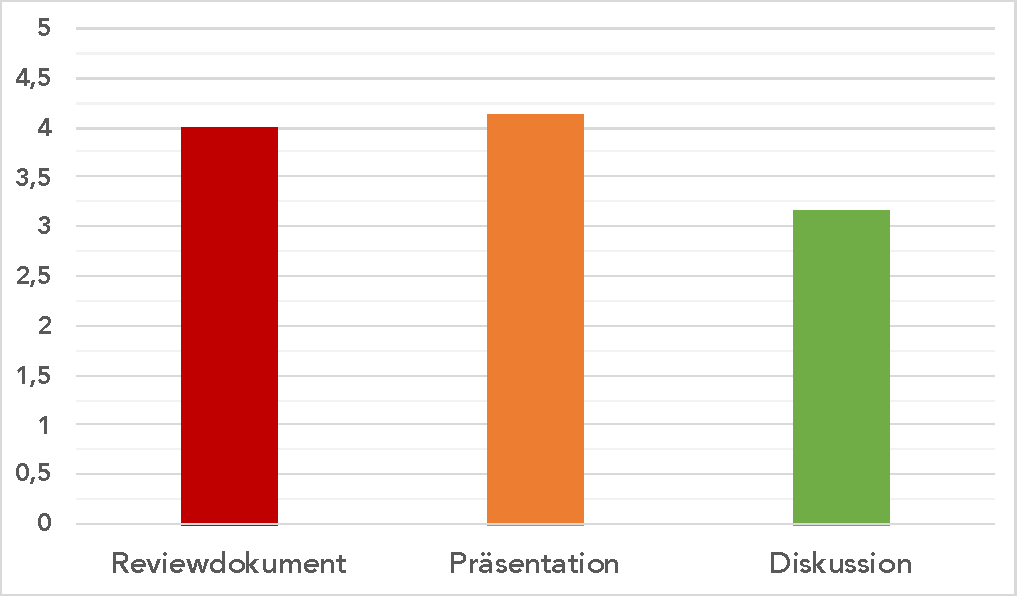
\includegraphics[width = 0.7\linewidth, trim=5pt 5pt 5pt 5pt, clip]{img/umfrageimplement.pdf}
    \caption{Implementierungsphase: Ergebnisse der Bewertung des Reviewdokuments, der Präsentation und der Diskussion im Anschluss}
    \label{implement}
\end{figure}
Etwas anders sieht es hingegen bei der Diskussion, die nach dem Vortrag stattgefunden hat, aus. Eine Einordnung von 3,17 besagt, dass die meisten Befragten nicht wirklich zufrieden gewesen sind. Ein Grund dafür ist vermutlich die nicht besonders treffende Beantwortung von Fragen, zum Beispiel nach dem Stand des Testens und des Prototyps. Hier hätte noch genauer geantwortet und überzeugter von bereits erledigter Arbeit berichtet werden können.

\begin{longtable}[H]{p{6,7cm} p{7,1cm}}
    \toprule
    \textbf{Frage}                     & \textbf{durchschnittliche Klassifizierung durch die Umfrageteilnehmenden} \\ \midrule \endhead
    Zeitliche und psychische Belastung & 2,625                                                                     \\
    Verteilung der Arbeit              & 3,714                                                                       \\ \bottomrule
\end{longtable}

Wie aus der oben stehenden Tabelle abgelsen werden kann, wurde auf die Frage nach der zeitlichen und psychischen Belastung im Durchschnitt mit einem Wert von 2,625 geantwortet. Das heißt, dass sich dieser Wert im Vergleich zur Implementierungsphase leicht um 0,5 Punkte verbessert hat.

Ein ähnliches Bild zeichnet sich bei der Verteilung der Arbeit über die Projektphase hinweg ab. Mit 3,714 wurde im Durchschnitt abgestimmt, was eine leichte Verbesserung um ca. 0,3 bedeutet.

Die Verbesserungen resultieren bei einem Befragten zum Beispiel aus kürzer gehaltenen Meetings. Eine weitere Anmerkung besagt, dass die Motivation für das Projekt mit dem Verlauf stark schwankte.

\subsection{Validierungsphase}

Da zum Zeitpunkt der Umfrage und der Erstellung dieses Dokuments weder das Reviewdokument fertig gestellt worden war noch die Präsentation gehalten worden war, unterscheiden sich die Fragen bezüglich der Validierungsphase zu denen der zwei vorherigen Phasen. Die Antworten können auch in diesem Teilkapitel der folgenden Tabelle entnommen werden.

\newpage
%
%
%Vielleicht kann das newpage doch irgendwie vermieden werden!
%
%

\begin{tabular}[t]{p{6,7cm} p{7,1cm}}
    \toprule
    \textbf{Frage} & \textbf{durchschnittliche Klassifizierung durch die Umfrageteilnehmenden}\\ \midrule
    Zufriedenheit mit dem bisherigen Ergebnis des Projekts & 3,7\\
    Zeitliche und psychische Belastung & 2,3 \\
    Verteilung der Arbeit & 4,25 \\
    Zufriedenheit mit dem bisherigen Stand des Reviewdokuments & 5,0 \\
    \bottomrule
\end{tabular}

Alle Antworten beziehen sich auf den Stand vom 12.07.2021.

Die Zufriedenheit mit dem bisherigen Ergebnis des Projekts kann als mittelhoch bis hoch bezeichnet werden, denn die durchschnittliche Klassifizierung beträgt 3,7. Ein möglicher Grund dafür ist zum einen die Tatsache, dass nach monatelanger harter Arbeit zum Zeitpunkt der Umfrage fast ein fertiger Prototyp steht. Auf der anderen Seite wären einige Umfrageteilnehmenden vermutlich zufriedener, wenn noch mehr Anforderungen, die über die Muss-Kriterien hinausgehen, erfüllt werden würden. Ca. eine Woche vor Ende des Softwareprojekts sieht es allerdings danach aus, dass viele spannende Features, die zu Beginn nicht mit Must priorisiert wurden, letzten Endes nicht ihren Weg in das System finden.

Wie in der Tabelle zu entnehmen ist, bringt die letzte Phase des Softwareprojekts noch einmal eine höhere Belastung für die Teammitglieder mit sich als die Implementierungsphase. Der Wert 2,3 bewegt sich zwischen dem der beiden anderen Phasen. Gerade zum Ende des Projekts sind viele Änderungen und Verbesserungen nötig, während gleichzeitig ein großer Zeitdruck besteht, wodurch einige Studierende regelmäßig nach einem sowieso schon anstrengenden Tag noch eine Nachtschicht für die Arbeit am Projekt in Angriff nehmen müssen. Dieser und andere Faktoren führen schließlich zu einer fragwürdig starken Belastung über den gesamten Zeitraum des Projekts hinweg. Eine Person merkte an, dass vor allem die Suche nach diversen Fehlern sehr frustrierend sei.

Wichtig ist auch die Anmerkung, dass die Verteilung der Arbeit in dieser Phase so gut wie noch nie bewertet wurde. Der Wert von 4,25 entspricht einer Verbesserung von über einem halben Punkt im Vergleich zu Implementierungsphase. Das heißt, dass das Team im Laufe des Projekts dazugelernt hat und sich die Arbeit im Laufe des Projekts stetig besser verteilt hat. Eine bessere Verteilung ist sehr positiv zu bewerten, weil diese eine in den allermeisten Fällen eine geringere Belastung beziehungsweise eine höhere Produktivität mit sich bringt.

Zuletzt wurde nach der Zufriedenheit mit dem derzeitigen Stand dieses Dokuments gefragt. Zwar zeigt die Bewertung mit 5,0 zunächst eine sehr hohe Zufriedenheit, es muss dennoch angemerkt werden, dass lediglich zwei Teilnehmende bei dieser Frage abgestimmt haben, während es bei den anderen zu Enthaltungen kam. Womöglich haben sich einige Studierende aufgrund der intensiven Arbeit am System während der Validierungsphase noch nicht wirklich mit dem Reviewdokument beschäftigen können, weshalb sie keine unfundierte Antwort abgeben wollten.

\section{Weitere Ergebnisse aus der Umfrage}
In den Umfragen wurden daneben Fragen gestellt, die sich nicht in die Kapitel \glqq Kritische Bewertung des Projekterfolgs\grqq{} und \glqq Kritische Bewertung des Vorgehens\grqq{} einordnen lassen. Deshalb werden die dennoch relevanten Ergebnisse dieser Fragen hier näher beschrieben.

Unter anderem wurden die Umfrageteilnehmenden gefragt, ob sie das \textbf{vierte Semester als einen geeigneten Zeitpunkt für das Softwareprojekt} hielten. Dieser Aussage stimmten 5 Personen zu. Drei Weitere bejahten diese Aussage nicht. Dies liege unter anderem daran, dass sie neben dem Softwareprojekt zu viele andere Module in diesem Semester hätten. So sei dieses Semester übermäßig voll. Sie klagten darüber, dass sie auf weit über 30 Leistungspunkte, bei einer Person sogar auf 37 Leistungspunkte, in diesem Semester kämen. Dies führe zu einer enormen Anstrengung und gehe auf die Substanz, vor allem da die 20 Wochenstunden für acht Leistungspunkte auch einen hohen Aufwand darstellten. Eine andere Person war der Meinung, dass auch im sechsten Semester die meisten Studenten nicht auf ein praxistaugliches Projekt vorbereitet seien. So sei es ihrer Meinung nach unerheblich, ob das Projekt direkt im ersten oder erst im letzten Semester stattfinde.

Eine ähnliche Frage bezog sich darauf, ob die vom Studiengang abhängige \textbf{Anzahl an Leistungspunkten} (6 bzw. 8 LP) und der damit verbundene empfohlene \textbf{zeitliche Aufwand} (15 bzw. 20 Wochenstunden) als \textbf{angemessen} empfunden werde. Das Ergebnis von 2,875 (1: sehr unangemessen ... 5: sehr angemessen) kann so interpretiert werden, dass die Teilnehmenden die Anzahl an Leistungspunkte und den damit verbunden empfohlenen zeitlichen Aufwand als eher unangemessen empfanden. Es wurde kommentiert, dass das Projekt um einiges mehr Zeit in Anspruch nehme, da dieses nie als fertig betrachtt werden könne und sich somit praktisch dauerhaft mit diesem beschäftigen werden müsse. Zudem werde erwartet, dass die Studierenden sehr viel Zeit für das Projekt aufwenden, und das parallel zu einem als sehr voll empfundenen Stundenplan. Jemand war der Auffassung, dass der Aufwand für das Softwareprojekt viel größer als bei einem regulären 6/8-LP Kurs sei. Auch eine andere Person hielt es nicht für gut, dass hier für eine Lehrveranstaltung annähernd so viel Zeit aufgewendet wie für alle anderen Veranstaltungen zusammen werde. Hier wurde angemerkt, dass durch die 20 Stunden für das Softwareprojekt lediglich 20 Stunden pro Woche für die anderen Fächer übrig blieben (Annahme: Ein durchschnittlich intelligenter Student benötigt laut Prüfungsamtsmitarbeiterin IA 40 Stunden pro Woche, um allen Verpflichtungen des Studiums nachzugehen). Da diese restlichen 20 Stunden nicht ausreichen würden, hätte dieser Studierende mit einem Workload von über 80h/Woche zu kämpfen.

Die Frage \glqq \textbf{Wie fandest du die Unterstützung von den SSElern?}\grqq{} wurde ebenfalls gestellt. Der Ergebnis-Wert liegt bei 2,5 (1: sehr schlecht ... 5: sehr gut). Da der Anfang zum Teil als Sprung in das kalte Wasser empfunden wurde, würde sich eine Person etwas mehr Anleitung bzw. Begleitung wünschen. Ein anderer Teilnehmer merkte an, dass er zwar nicht im direkten Kontakt mit den Mitarbeitern des Fachgebiets System- und Software-Engineering stand, aber er die Antworten auf Fragen als sehr schwammig und wenig hilfreich empfand.  Verbesserungswünsche beziehen sich zudem auf die Übersichtlichkeit des Moodlekurses und der Kompromissbereitschaft bezogen auf die Wahl des Projektthemas mit externen Beratern. Positiv wurde angemerkt, dass zügig auf Fragen reagiert wurde.

Die \textbf{Unterstützung des Fachgebiets Telematik/Rechnernetze} wurde mit 4,25 bewertet (1: sehr schlecht ... 5: sehr gut). Dieser gute Wert ist vor allem dem Betreuer des Projektes hinzuzurechnen, was Kommentare wie \glqq Martin ist der Beste!\grqq{} zeigen. Die Kommunikation mit ihm wurde als sehr gut bewertet, er sei stets erreichbar gewesen und habe allen bei schwierigen Fragen unterstützt. Ebenso sei die Arbeit durch ihn sehr gut organisiert gewesen. So wurden gleich zu Beginn Rollen vergeben und Vorträge sollten vorbereitet werden. Auch bei den Review-Dokumenten und den Vorträgen habe er konstruktiv kritisiert und es wurde noch einmal Druck gemacht, wenn etwas nicht so gut war. So habe dies nochmal das Beste aus dem Team herausgeholt. Zudem habe er auch bei schwierigen Fragen, insbesondere beim Programmieren, das Team stets unterstützt. Das sei vor allem deswegen gut, da die Teilnehmenden vorher keine ausführliche Programmiererfahrung im Studium hätten. Auch eine andere Person meinte, dass ohne Martins Hilfe der Projektfortschritt viel geringer ausgefallen wäre. Was ebenfalls zu einem so positiven Ergebnis beitrug, war das Angebot des Hostens einer Website für 2 Jahre. Ein weiterer Kommentar besagte Folgendes: \glqq Martin nahm sich Zeit für meine Probleme und leistete Unterstützung bei fachlichen und allgemeinen Fragen.\grqq{}

Die Teilnehmer wurden auch gefragt, welche Dinge ihnen besonders \textbf{Spaß} gemacht haben.
Zum einen war dies das Arbeiten im Projekt und als Team , aber auch die gemeinsamen Meetings. Zum anderen wurden das Programmieren, die Freude, wenn etwas nach langem Testen funktioniert hat, und das Lernen von Neuem, vor allem im Bezug auf C++, von vielen als Spaß empfunden. Einige fielen auch Gefallen an der Aufwandsschätzung, am Schreiben der Reviewdokumente und am Halten von Präsentationen.

Nach den Ergebnissen der Umfrage hat aber vor allem der hohe Zeitaufwand, und teilweise  Zeitdruck, den Teilnehmern \textbf{keinen Spaß} gemacht. Auch die Suche von Fehlern, die Dokumentation, die Wartezeiten auf die Fertigstellung anderer Komponenten oder die Installation wurden hier geäußert. Während für manche die Implementierung Spaß machte, waren andere wiederum gegenteiliger Meinung.

Teilweise scheinen die Punkte, die Spaß bzw. nicht Spaß gemacht haben, konträr. So wurde beispielsweise von einigen das Programmieren als spaßig empfunden, von anderen wiederum nicht. Dies ist unter anderem auf die individuelle Wahrnehmung und Interessen der einzelnen Teammitglieder zurückzuführen.

Die Umfrage beinhaltete überdies eine Frage, bei welcher die drei wichtigsten Dinge aufgezählt werden sollten, welche die Person \textbf{während des Softwareprojektes gelernt} habe.
Es wurde von beinahe allen Teilnehmern aufgeführt, dass sich deren Programmierkenntnisse verbessert haben, insbesondere im Bezug auf die vorwiegend verwendete Programmiersprache C++. Zusätzlich habe sich der Schreibstil bei einer Person verbessert. Auch der Umgang mit der Versionsverwaltungssoftware git, dem Betriebssystem Linux, das Lesen von Dokumentation und des Erlernen von Latex-Grundlagen wurden positiv bewertet. Das Erlangen von Projekterfahrung und praktischer Umgang mit Projektmanagement sehen einige als einen wichtigen Gegegenstand. So wurde auch praktisch erlernt, wie effizientes Arbeiten in der Gruppe gewährleistet werden könne. Das heißt zum Beispiel, wann es wichtig sei, ein bestimmtes Thema anzusprechen oder wann dieses lieber übersprungen werden sollte.
So musste zudem der Prozess der Software-Entwicklung praktisch komplett durchlaufen werden und ein ganzes Projekt mit Planung und Entwurf umgesetzt werden. Innerhalb des Projekt habe sich auch gezeigt, dass sich Anforderungen schnell wechseln können. Es wichtig sei, von Anfang an feste Grenzen festzulegen. Auch die Relevanz der Kommunikation (u.a. mit Mitarbeitenden) sei durch das Projekt deutlich geworden.
Zudem erlangte das Team Wissen über (D)Dos-Attacken.

Eine weitere Frage lautete: \glqq \textbf{Inwiefern hat sich das Softwareprojekt von deinen Erwartungen unterschieden?}\grqq{}.
Einen Teilnehmer empfand den Verlauf dieses Softwareprojekts als ziemlich gut, wenn er es mit den Erzählungen verglich, die er zuvor gehört habe. Bei diesen Erzählungen wurde über schlechte Kommunikation und Organisation geklagt. Jemand anderes war der Meinung, mit dem Betreuer sehr viel Glück gehabt zu haben. Denn ohne diesem hätte das Team nicht so gut gewusst, welche Aufgaben es zu welchem Zeitpunkt und auf welche Art und Weise hätte bearbeiten sollen. Er erwartete weiterhin, dass am Projektbeginn mehr Anleitung bzw. Begleitung von den Mitarbeitern des Fachgebiets SSE eingeplant sei. Bei einer wiederum anderen Person unterschieden sich ihre Erwartungen überhaupt nicht von der Realität. Es sei genauso durcheinander, chaotisch, ungeplant und unfertig, wie sie es vermutet habe. Der Nächste wiederum empfand das Projekt als deutlich komplizierter als erwartet. Seiner Meinung nach sei außerdem die Rollenzuteilung teilweise irrelevant gewesen. Zudem habe er mehr Gruppenarbeit erwartet. Eine weitere Person hatte trotz des enormen Zeitaufwands viel Spaß. Von drei anderen wurde angemerkt, dass das Projekt deutlich mehr Aufwand und Zeit in Anspruch nehme als zunächst geschätzt. So sei aber auch das Thema mit etwas mehr Fallstricken und Schwierigkeiten besetzt als erwartet und das bei anderen Projekten der Fall sei.
\end{document}
